\documentclass[twoside]{uva-inf-bachelor-thesis}
%\usepackage[dutch]{babel}

% Filling your thesis with only lorem ipsum is not advised.
\usepackage{lipsum}
\usepackage{listings}

% Citations
\usepackage[style=numeric]{biblatex}
\addbibresource{references.bib}

% Title Page
\title{Improving government transparency with a video search engine}
\author{Pepijn van Wijk}
\supervisors{Dr. Maarten Marx}
\signedby{Signees}

\begin{document}
\maketitle

\begin{abstract}
\lipsum[2]
\end{abstract}

\tableofcontents

\chapter{Introduction}
One of the foundations of a strong democracy is transparency. Citizens must have the opportunity to be informed about- and control the inner workings and decision making process of their (local) governments. To help improve government transparency, Dutch lawmakers introduced the 'Wet Open Overheid' (Woo) \footnote{https://wetten.overheid.nl/BWBR0045754} in 2022. 
This law is applicable to all governmental bodies, from the house of representatives to local municipalities to the tax authority. The three most important terms the Woo brings are: \textit{active publication}, stating government bodies should actively publish some types of information. \textit{Publication on request} states that information should be made public on request. Lastly, the \textit{information management obligation} states that all this information should be easily accessible. 

Various online tools such as the official Woo-index \footnote{https://organisaties.overheid.nl/woo} and Woogle \footnote{https://woogle.wooverheid.nl} offer the ability to search through a wide range of uploaded documents and information. 
Though millions of documents are already publishes and searchable, the searchability of one important type of information is lacking; the meetings. Decisions, from large to small, are made during long meetings that are livestreamed and archived. These video archives, often three to four hours, not only require vast amounts of storage, they are also difficult to comb through. 
Imagine a journalist writing an article about a new piece of legislation that was, among other things, debated the night before by the local municipality. They want to write what the different parties think of the bill and how they voted. Currently, they would have to watch or skip through to video until they find the part where they talk about the proposed law. Then, they would have to watch the debate and take notes on what each Representative argued, along with their arguments.  Understandably, this simple sounding process quickly becomes both time consuming and inefficient. 

This research provides a solution to this issue by answering the question \textit{how can AI be utilized in order to increase information retrievability of large video archives, in particular of democratically elected councils}? In order to land at a satisfying answer to this research question, some related questions need to be answered first. 
First, the video archives need to be obtained. This means that the first part of this research will be finding an answer to the question \textit{what are the different archive formats local authorities host in order to comply with the Woo and how are these formats exploited to retrieve as much information as possible}?
To extract as much relevant information from the video archives, the question \textit{what state-of-the-art audio analysis tools can be used to improve searchability of the meetings}? needs to be answered. During the aforementioned hour long meetings, many different subjects are discussed. By answering the question \textit{how accurately can such a video be segmented into the meaningfully different parts which are discussed}?, this fact can be used to provide a better overview of the video, as well as enhancing searchability. Finally, an answer to the question \textit{what state-of-the-art information retrieval techniques can be leveraged to develop an efficient video information retrieval system}? should be found, tying everything together.
On top of these base questions, the last part of this research regards an integration of the search system with a large language model, answering the final sub question \textit{how well can the developed search system be integrated with a large language model, creating a helpful chat bot capable of answering questions and providing complementary information when needed}?

\chapter{Related work}
The act of archiving and transcribing parliamentary meetings is not new. Most big governmental organisations such as the European Parlement and the Dutch House of Representatives host an online archive that offers an elementary search mechanism. 
These online archives offer a pleasant viewing experience, showing the current speaker and what is being said. Most of the time, the active speaker is not automatically detected, but the information is taken from the currently active microphone, which is linked to a person. Occasionally, this results in an incorrect speaker being highlighted when the speaker speaks through a different microphone than they were assigned.
On top of this, the search functionalities that these existing archives offer is often limited to a naive keyword search comparable to a control+f search, or they offer no searching at all.

Some proprietary tools provide users the ability to search specifically through (AI generated) meeting notes. The main purpose of these tools generally is the generation of notes, not the searching. As a result, the search mechanism is a simple keyword search, showing all text snippets containing the given query. 

Stepping away from searching through meeting video archives,previous studies have explored the searching of video archives containing online lectures. The majority of these studies use a combination of transcripts and optical character recognition (OCR) obtain relevant search results, leveraging the fact that on-screen text has a high probability of being relevant to the discussed subject \cite{Adcock10, yang14}. 
Unfortunately, this approach won't work for searching through parliamentary meetings since these meetings held without an accompanying screen that is showing information. 

\chapter{Theoretical background}

\section{Natural Language Processing}
Natural Language Processing (NLP) is the field in computer science primarily focusing on enabling computers to understand human language. Naturally, simply having knowledge of different words and their meaning does not suffice for achieving this goal. A true understanding of language can only be obtained by understanding grammatical rules, contextual details and potential informal vernacular differences in texts from different areas.

% Natural language processing is widely used in everyday life. Whenever you see a foreign article on the internet and use the translate feature to translate this text to English for example. Or, blabla bla bla...

Natural language processing has its historical roots roughly halfway of the previous century. During this time, early experiments were performed trying to create computer chat bots and to automatically translate foreign languages. From the 1950's onwards, an approach that is now called 'symbolic NLP' was used. Symbolic NLP is similar to the way humans learn to understand languages: using a set of handcrafted rules, structures, patterns and decision trees, a framework for the understanding and generation of a language is created. The machine then follows this set of rules to determine the desired output \cite{Dale00}. One example of this symbolic NLP approach is the ELIZA computer program, dating back to 1964. ELIZA was developed by Joseph Weizenbaum at MIT. ELIZA analyzes input sentences by applying a set of generated decomposition rules and key word detection \cite{weizenbaum66} \cite{Jurafsky08}. A response is then generated by a rule set focused on mimicking Rogerian psychotherapy responses \footnote{For more information, see Yao, 2023. \cite{Yao23}}. 

\begin{figure}[h]
    \begin{verbatim}
    [User]:  Men are all alike.
    [ELIZA]: IN WHAT WAY?
    [User]:  They're always bugging us about something or other. 
    [ELIZA]: CAN YOU THINK OF A SPECIFIC EXAMPLE?
    [User]:  Well, my boyfriend made me come here.
    [ELIZA]: YOUR BOYFRIEND MADE YOU COME HERE?
    [User]:  He says I'm depressed much of the time
    [ELIZA]: I AM SORRY TO HEAR YOU ARE DEPRESSED
    \end{verbatim}
    \caption{A piece of conversation with ELIZA. \cite{weizenbaum66}}
    \label{fig:eliza-conv}
\end{figure}


With the rapid advances of computational power, the lessening of the dominance Noam Chomsky's linguistics theories and the greater digitisation of written texts, the 80's brought in a natural language processing revolution. The old system of rule sets and decision trees was replaced by a new approach using statistics and machine learning. Instead of following a set of rules, statistical NLP focuses on the identification of common patterns found within a given corpus of language \cite{Manning99}. The detection of these patterns is learned from gigantic bodies of text, called a corpus (plural: corpora). The popularization of the internet and various governments' efforts of digitisation greatly facilitated the collection of these corpora. 
Perhaps the best example of an application of statistical NLP is the predecessor of all current state-of-the-art large language models, the n-gram language model. The n-gram language model works by predicting the occurrence of a word, based on the preceding $n-1$ words. The probability of a word $w_n$ occurring at the end of a sequence of words $w_{n-N+1 : n-1}$ is given by equation \ref{mle} \cite{brown92, Manning99}.
\begin{equation} \label{mle}
    P(w_{n} | w_{n-N+1 : n-1}) = \frac{C(w_{n-N+1 : n-1} w_{n})}{C(w_{n-N+1 : n-1})}
\end{equation}
Here, $N$ is the window of text and $C$ is the count of occurrences, as found in the corpus. 

Naturally, large amounts of text need to be processed in order to form an accurate probabilistic model. Despite being first invented in 1948 by mathematician Claude E. Shannon \cite{shannon48}, the lack of computational power to process these large amounts of text prevented the implementation of the n-gram model until much later.


For many years, the n-gram language model was the state-of-the-art algorithm in language processing. Despite this, it had a significant problem: the curse of dimensionality. The curse of dimensionality is the exponential growth of computational resources needed, when dimensionality of discrete variables increases. To illustrate this, let's say one wants to model the joint distribution of $10$ consecutive words in a language with a vocabulary V of size $100,000$. The amount of free parameters here would total $100,000^{10}-1 = 10^{50}-1$ \cite{bengio03}. 
In 2003, Youshua Bengio et al. proposed a new method of predicting the next word given a sequence of preceding words, utilizing a multi-layer perceptron. Instead of raw strings, it makes use of dense vector representations of words, with semantically similar words embedded closer to each other than meaningfully different words. The continuous nature of these word embeddings inherently do not suffer from the dimensionality curse, since probabilities for (unseen) word sequences are based on the learned similarities between similar vectors. These word feature vectors and the parameters of the probability function are learned during the processing of the training corpus \cite{bengio03}. This innovation gave birth to the current most popular approach to natural language processing: neural NLP.

% Iets over dat strings niet gebruikt worden, maar tokens en word- en sentence segmentation en tokenization enzo (?)
\subsection{Word feature vectors}
As briefly described in the previous section, current state-of-the-art NLP techniques works with embeddings of text. Despite being introduced in the early 2000's, this method did was not successful at corpora containing more than a few hundred millions unique words. In 2013, Google introduced Word2vec, alongside a paper proposing several techniques to train and obtain high quality word vectors, with a larger vocabulary and more accurate than before \cite{mikolov13}.


\begin{figure}
    \centering
    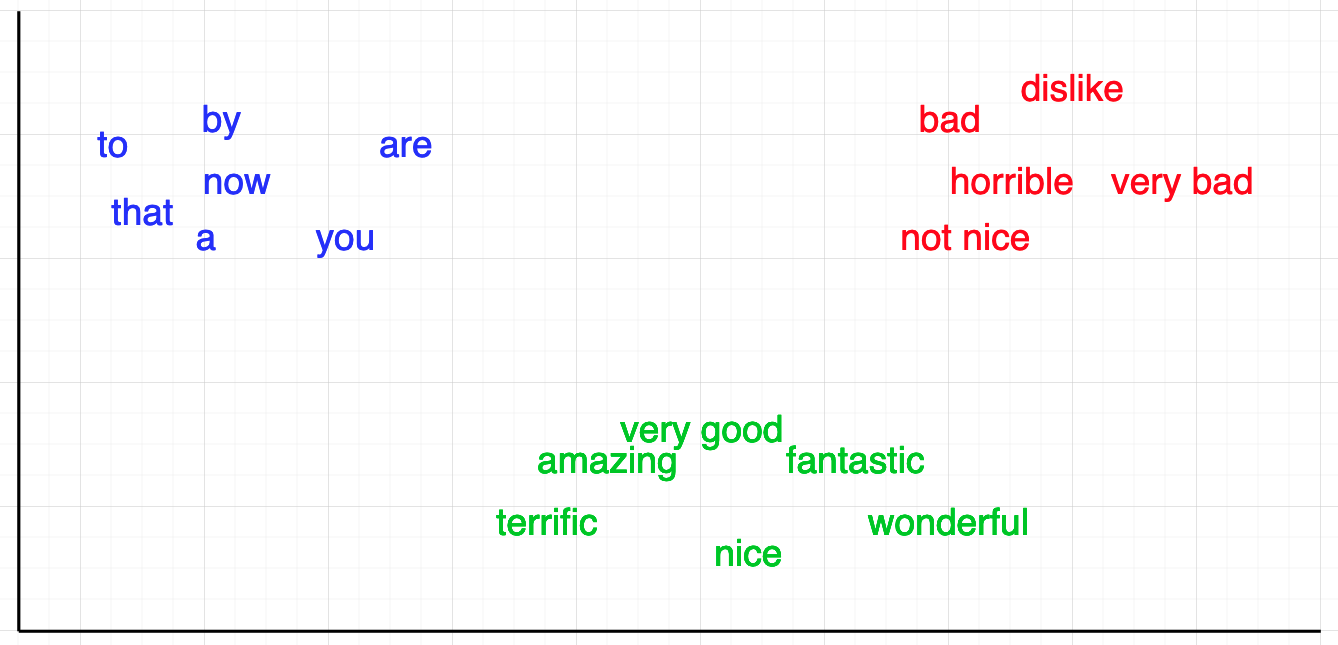
\includegraphics[width=0.85\textwidth]{images/embeddings.png}
    \caption{A two-dimensional (t-SNE) projection of word embeddings. Adapted from \cite{Manning99} and \cite{li16}}
    \label{fig:embeddings}
\end{figure}

Interestingly, these vector representations contain an embedded meaning of the word. As stated before, semantically similar words are embedded close to each other in the vector space, a schematic, 2D representation of this phenomenon is illustrated in figure \ref{fig:embeddings}. Besides this locality, word vectors also contain relationships to other words, as learned from the context provided by the dataset. Perhaps the most famous example of this was found by one of the authors of Word2vec, several years earlier \cite{mikolov13_2}. This paper showed that when the vector representing 'Man' ($V('man')$) was deducted from $V('king')$, the result of which added to the vector $V('woman')$, results in a vector closest to the word 'Queen'. Later, the Word2vec paper presented several other examples showing the capabilities of 'word vector arithmetic', as seen in figure \ref{fig:vecarith}.
\begin{figure}[h]
    \centering
    $$V('copper') - V('Cu') + V('zinc') \approx V('Zn')$$
    $$V('Einstein') - V('scientist') + V('Mozart') \approx V('violinist')$$
    $$V('Japan') - V('sushi') + V('Germany') \approx V('bratwurst')$$
    \caption{Word vector arithmetic examples (interpreted as 'zinc is to ... what copper is to Cu'). From \cite{mikolov13}}
    \label{fig:vecarith}
\end{figure}

\subsection{Contextual feature vectors}

Since the end of the 2010's, the implementation of Word2vec is not considered state-of-the-art anymore, being replaced by BERT \cite{devlin19} and GPT \cite{brown20}. The introduction, and consequent improvements of the transformer model shifted the focus in NLP to the utilization of these transformer models. Transformer models are like regular neural networks, but add several so called 'attention layers', allowing words to be processed in relation to all other words in the sequence, taking the specific context into account \cite{vaswani17, vondermosel22}.
% TODO: meer uitleggen over contextual en trasnformers, dit is wat ik gebruik, MPnet paper aanhalen 

\section{Information retrieval} \label{retrievalSection}
According to current Director of the Stanford Artificial Intelligence Laboratory Christopher Manning, information retrieval can be defined as: 

\say{Information Retrieval (IR) is finding material (usually documents) of an unstructured nature (usually text) that satisfies an information need from within large collections (usually stored on computers).}\cite{manning08IR}

This definition steps away from the historic way of searching for data using database systems. In such systems, specific (unique) identifying information such as an order ID or document ID is needed to find data from an information system. Perhaps the most used manifestation that encapsulates this modern way of looking at IR is the Google search engine. The user enters a query, which attempts to communicate the user's information need. The search engine then performs various IR algorithms and ranks results based on their relevance to the entered query. Before the documents can be searched and ranked, they need to be pre-processed. In a process called indexing, a universal representation for the documents is derived that the system can efficiently index.

\begin{figure}[h]
    \centering
    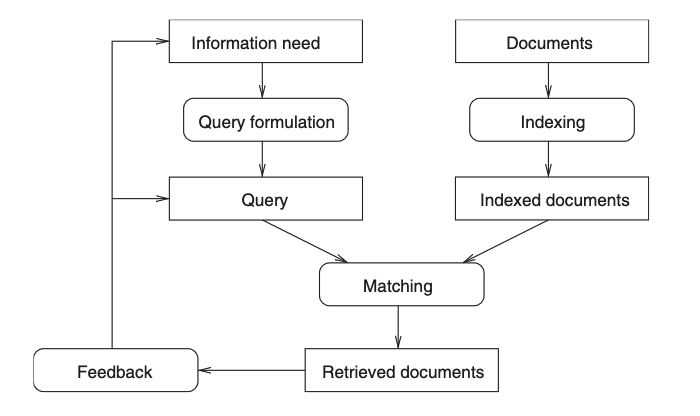
\includegraphics[width=0.85\textwidth]{images/irDiagram.png}
    \caption{Information retrieval process. From \cite{goker2009information}}
    \label{fig:ir}
\end{figure}

Over the years, many different approaches to IR came forward. These different strategies are roughly categorized in three separate models: the boolean model, the probabilistic model and the algebraic model. \cite{goker2009information}

\subsection{Boolean information retrieval}
The boolean model employs a relatively simple and straightforward strategy to information retrieval. A query consists of search terms and potentially the mathematical logical operators AND, OR and NOT. A search term either matches a document, or it does not. Thus, search results can not ranked be ranked like in other models.\cite{goker2009information, manning08IR} An example query that looks for political documents containing the term 'China', but not 'Japan' could look like the following, for example.
\begin{verbatim}
    political AND contains(China) AND NOT contains(Japan)
\end{verbatim}
Due to the fact that boolean queries lack the ability the rank returned results, this model is rarely used in practice. Other models that can rank results and offer the user more freedom to construct searches are favoured in modern systems.

\subsection{Algebraic information retrieval}
The algebraic model facilitates ranked retrieval, in which there is a collection of documents (the corpus), the user issues a query, and a ranked list of documents relevant to the query is returned.

Assume the collection of documents has been pre-processed and indexed into many vectors as described in section \ref{}. Recall that semantically similar words and sentences lie closer in vector space than semantically dissimilar text. Given this fact, similar documents will naturally lie close to each other. Additionally, embedded queries that are relevant to specific documents, will be embedded relatively close to these relevant documents, meaning the measure of similarity between two vectors can function as a ranking score.

The two most popular ranking functions are \textit{Euclidean distance} and \textit{cosine similarity}. Euclidean distance is a widely used metric in clustering problems, measuring the distance between two points in space. Equation \ref{eq:eucDist} gives the general formula for calculating the euclidean distance between two vectors $\textbf{V}$ and $\textbf{W}$ of dimension $n$. \cite{huang2008similarity}
\begin{equation}\label{eq:eucDist}
    D(\textbf{V}, \textbf{W}) = \sqrt{\sum_{i=1}^{n} (V_{i} - W_{i})^{2}}
\end{equation}
Cosine similarity, given in in equation \ref{}, is more popular in textual document information retrieval systems. It is not a metric of distance, but how similar two vector represented documents are. Similarity here, is seen as the angle between two vectors. Thus, unlike Euclidean distance, the difference in magnitude of two vectors has no influence on the metric. \cite{huang2008similarity, rahutomo2012semantic, manning08IR}
\begin{equation}\label{eq:cossim}
    S(\textbf{V}, \textbf{W}) = \frac{\textbf{V} \cdot \textbf{W}}{\lvert \textbf{V} \rvert \times \lvert \textbf{W} \rvert}
\end{equation}

Now, with a means of ranking documents based on a user's query, a search through the corpus is possible. However, the computational complexity to perform a search through all documents scales linearly with the documents. This means that large corpora will quickly become infeasible to query \cite{malkov2018efficient}.

\subsection{Probabilistic information retrieval}
Another model facilitating ranked retrieval is the probabilistic model. Central to this model lies the Probability Ranking Principle (PRP):

\say{If a reference retrieval system’s response to each request is a ranking of the documents in the collection in order of decreasing probability of relevance to the user who submitted the request, where the prob- abilities are estimated as accurately as possible on the basis of what- ever data have been made available to the system for this purpose, the overall effectiveness of the system to its user will be the best that is obtainable on the basis of those data.} \cite{robertson1977probability}

The main challenge of probabilistic information retrieval, is finding a ranking function that efficiently provides an accurate ranking of documents in a collection. 
% TODO over Binary Independence Model

\subsubsection{Okapi BM25}
TODO


\subsection{Vector databases}
Vector databases are a relatively new technology that offer a storage and retrieval mechanism optimized for enormous amounts of data, often capable of querying hundreds of millions of documents with only milliseconds latency. 
These remarkable results are achieved by the use of approximate nearest neighbor (ANN) algorithms, offering some accuracy for for a large speed gain \cite{han2023comprehensive}. 

\subsubsection{Hierarchical Navigable Small World graphs}
One of the most employed ANN algorithms is Hierarchical Navigable Small World graphs (HNSW) \cite{malkov2018efficient}. This proximity graph based algorithm is TODO

\subsubsection{Hybrid search}
Many vector databases allow for a combination between ANN powered vector similarity search and probabilistic searches. todo balblalba...


\section{Video \& audio analysis}
Before any of the aforementioned processing and retrieval can be performed, the video must be analysed and pre-processed. As deduced from the stated research questions, the main analysis and processing that is mandatory is transcription, with the use of automatic speech recognition tools, speaker detection, which is done with speaker diarisation models and topic segmentation with the use of large language models.

\subsection{Automatic Speech Recognition}
Automatic Speech Recognition (ASR), informally known as Speech To Text (STT), is the act of transforming spoken language into written text by a computer. ASR has been an old problem, going through many different stages and bringing many technical innovations over the years. 
In the last two decades, the technical advances in ASR led to many consumer products used daily by tens of millions of people such as Amazon's Alexa and Google's home speakers.

One of the very first systems systems capable of recognizing speech was developed in the early 1950's by a research group at Bell Labs. The system was capable of recognizing ten different words: the numbers one through nine - and zero ('oh'). By measuring the spectral peaks resulting from the resonance of the human vocal tract during vowel sounds, known as formant frequencies (figure \ref{fig:ff}), for each digit, the known words could be recognized with an accuracy of 97\% to 99\%. One limitation was that these accuracies could only be reached after preliminary analysis of the speaker's voice. \cite{davis1952automatic, Juang05}

\begin{figure}[h]
    \centering
    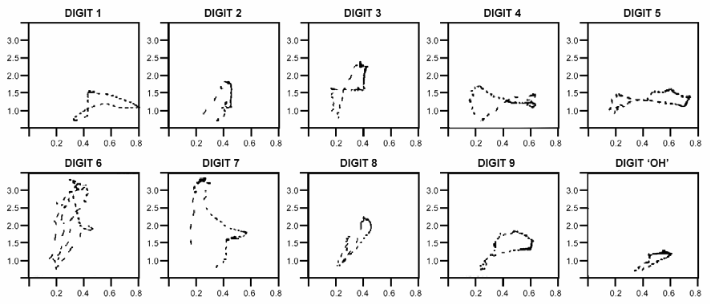
\includegraphics[width=0.9\textwidth]{images/formantFrequencies.png}
    \caption{Photographs of formant frequency presentations of the recognized digits. From \cite{davis1952automatic}}
    \label{fig:ff}
\end{figure}


From the late seventies onwards, a focus on statistical approaches gained traction in favor of the previously used pattern recognition methods. With the use of recently formulated Markov chains and hidden Markov models, subsequent systems rapidly grew to a vocabulary of a thousand word, which was later broken by IBM's Tangora system, capable of recognizing over 20,000 words. \cite{Juang05}

One particularly large milestone was the Sphinx-II system, developed in 1992 by, among others, Xuedong Huang at Carnegie Mellon University. Sphinx-II, using an advanced statistical approach, was the first system that had both a large vocabulary, and the ability to perform speaker-independent detection. The Sphinx-II also won DARPA's speech benchmark evaluation in 1992. ASR systems are mainly evaluated by their Word Error Rate (WER) (equation \ref{eq:wer}). Sphinx-II only suffered from a fairly low error rate of 5\% \cite{huang1993overview, huang2014historical}.

\begin{equation} \label{eq:wer}
    WER = \frac{S + D + I}{S + D + C}
\end{equation}
where: \\
\begin{conditions}
 S     &  the number of substitutions \\
 D     &  the number of deletions \\   
 I     &  the number of insertions \\
 C     &  the number of correct words
\end{conditions}

Up until the late 2000's, the use of hidden Markov models and similar statistical methods still dominated in the ASR space. However, with the advent of deep neural networks (DNNs) and the aforementioned transformer architecture, the paradigm has shifted yet again, bringing light the the current state-of-the-art: OpenAI's Whisper ASR.

\subsubsection{Whisper}
In 2022, OpenAI released Whisper, capable of 'Robust Speech Recognition via Large-Scale Weak Supervision' \cite{radford2023robust}. Trained on 563,000 hours of labeled English speech, and 117,000 hours of labeled speech in 96 different languages, Whisper is the current state-of-the-art ASR system, with a (post normalisation) word error rate that is similar to a professional human transcriber, as seen in figure \ref{fig:whisperwer}.
Whisper makes use of an encode-decoder Transformer, as described in \cite{vaswani17}. Input audio is first resampled and standardized, after which it is converted to a Mel Spectrogram, normalized and fed in to the network. A full view of the simplified architecture can be seen in figure \ref{fig:whisperarch}.

\begin{figure}
    \centering
    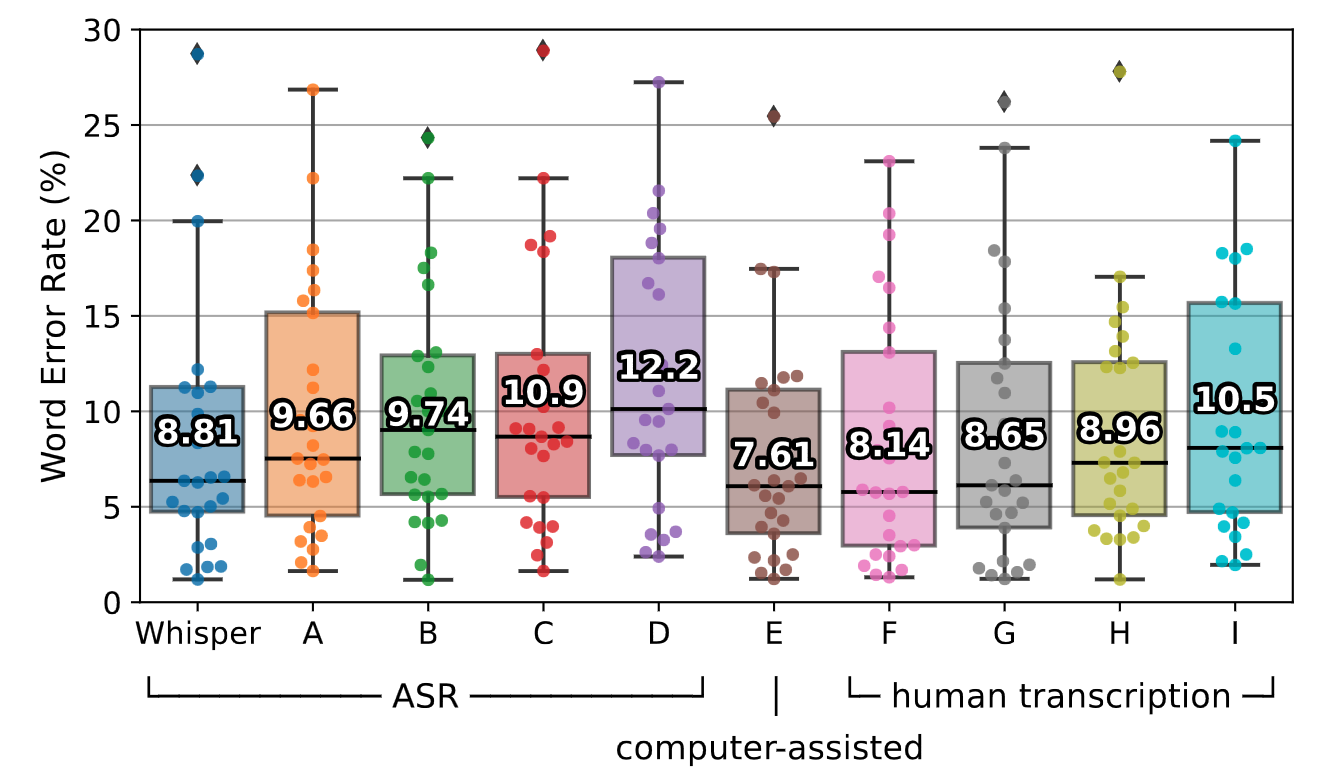
\includegraphics[width=0.8\textwidth]{images/whisperwer.png}
    \caption{Whisper WER compared to other companies and human professionals. From \cite{radford2023robust}}
    \label{fig:whisperwer}
\end{figure}

\begin{figure}
    \centering
    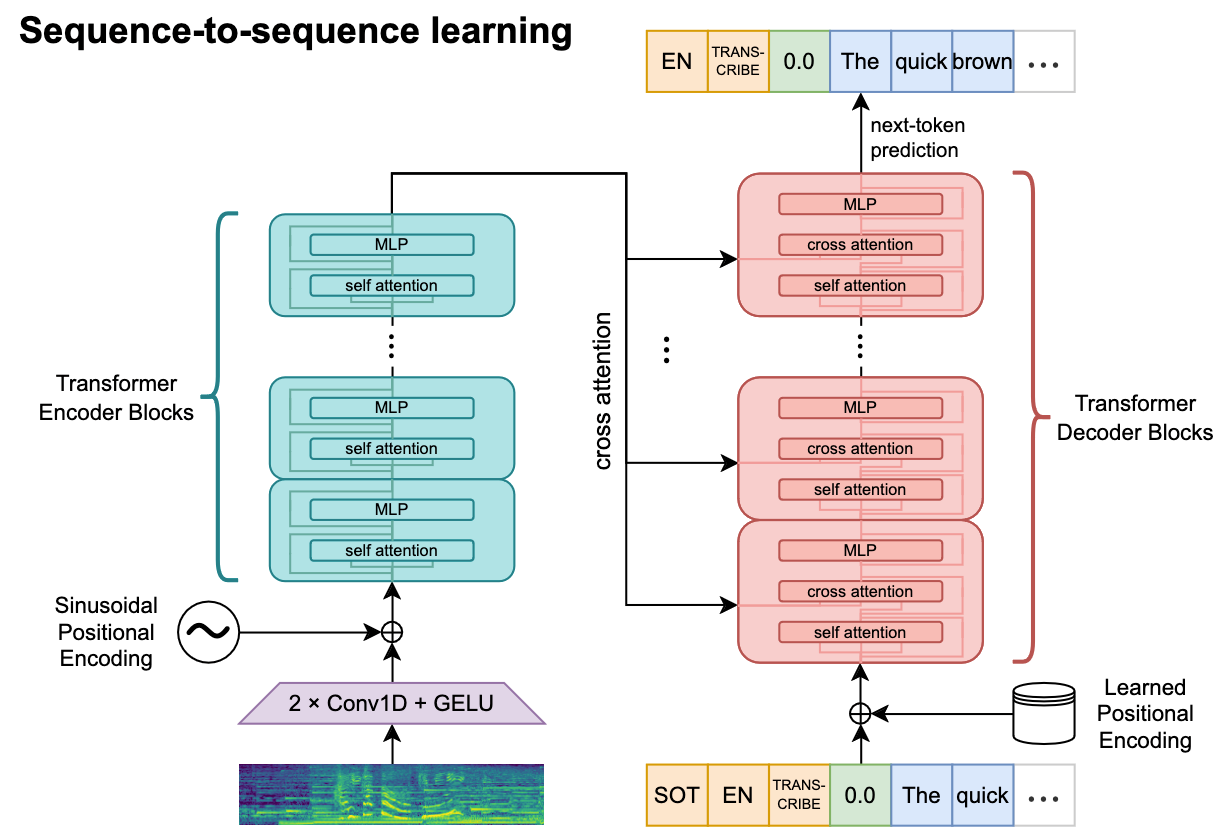
\includegraphics[width=0.9\textwidth]{images/whisperarch.png}
    \caption{Simplified Whisper architecture. From \cite{radford2023robust}}
    \label{fig:whisperarch}
\end{figure}

\subsection{Speaker diarisation}
Speaker diarisation (SD) is the process of partitioning input audio containing multiple speakers, in to separate segments containing single speakers. It aims to solve the question 'Who spoke when?' \cite{sahidullah2019speed}. Speaker diarisation is a relatively new problem. In film and news studios the central question is not necessarily a mystery; different speakers have different microphones, whose data is known and separate at the time of processing and editing. 

\begin{figure}[h]
    \centering
    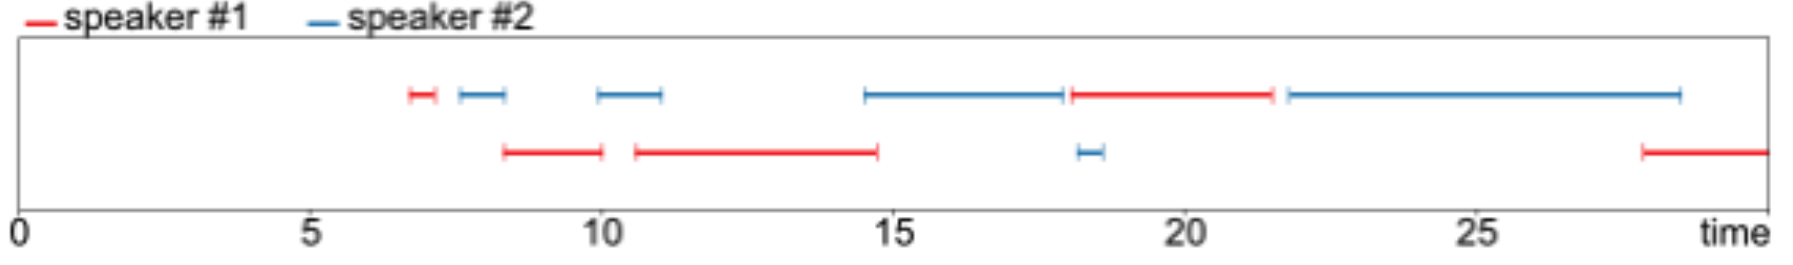
\includegraphics[width=0.75\textwidth]{images/speakerdiaroutput2.png}
    \caption{Desired speaker diarisation result. From \cite{bredin2023pyannote}}
    \label{fig:sdo}
\end{figure}

Central to speaker diarisation is voice profile feature extraction. When a reliable and accurate method of embedding voice profiles is achieved, these voice profile vectors can be compared using similarity measures such as cosine similarity or euclidean distance to find different speakers and when they speak. Different systems utilize different methods of obtaining feature vectors. Most of these feature extractors use various representations of sound waves, with additional features derived from pitch information and audio metadata, mostly from the standardised MPEG-7 audio standard \cite{kotti2008speaker, lu2002speaker}. Some of the most common features have a similar accuracy, Mel-frequency cepstral coefficients
(MFCCs) \cite{gook04} and Line spectral pairs (LSPs) \cite{lu2002speaker}. 

\subsection{Pyannote}\label{sec:pyannote}
 Pyannote.audio (pyannote) is the current state-of-the-art speaker diarisation mode. It is not only a speaker diarisation model, but it also offers a range of speaker diarisation sub-modules. These submodules include voice activity detection, overlapped detection speech, speaker change detection, and more. \cite{bredin2020pyannote, bredin2023pyannote}

In most competitions, speaker diarisation accuracy is graded by four criteria: speaker confusion rate (CONF), which is the duration of speaking where the speaker is mislabeled, false alarm rate, which is the duration of non-speech incorrectly classified as speech, missed detection, which is the duration of speech that is incorrectly classified as non-speech and Diarisation Error Rate (DER), which is the sum of these three. As can be seen from figure \ref{fig:pyanres}, pyannote scores at the top of most benchmarks. Top benchmarks are greatly improved by their preview baseline, while DERs on benchmarks where pyannote does not score at the top are fairly close, indicating a great overall performance. \cite{bredin2023pyannote}


The pyannote system uses the following distinct steps on five seconds sliding windows of audio \cite{bredin2023pyannote}: 
\begin{enumerate}
    \item Local speaker segmentation, where these windows are analysed for different speakers and when these different speakers start- and stop speaking.
    \item Local speaker embedding, where the voice profiles of the different speakers in the sliding windows get embedded.
    \item Global agglomerative clustering, where local speakers are grouped into global clusters. 
\end{enumerate}

Pyannote diarisation outputs are formatted according to the Rich Transcription Time Marked (RTTM) file format, described in \cite{ryant2018first}.

\begin{figure}
    \centering
    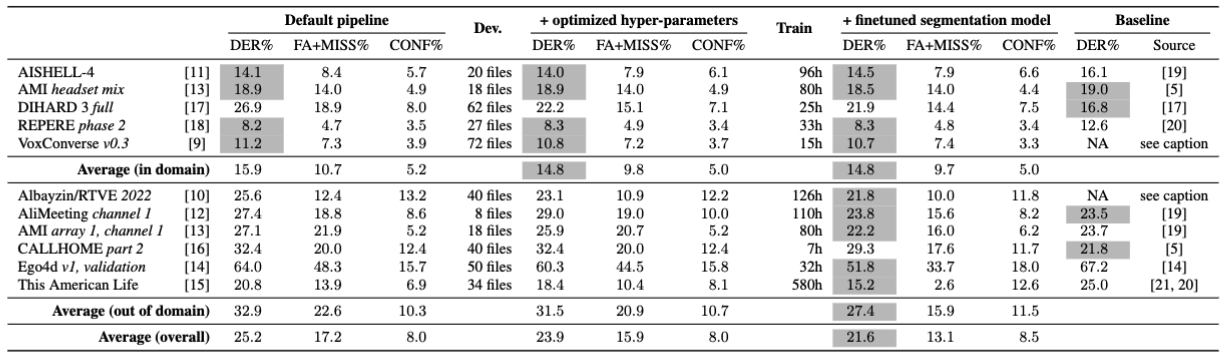
\includegraphics[width=0.99\textwidth]{images/pyanresults2.png}
    \caption{Performance of the (default, optimized, and fine-tuned) pipelines on 11 different benchmarks. The grey background marks the best results for each dataset as well as those less than 5\% worse relatively. From \cite{bredin2023pyannote}}
    \label{fig:pyanres}
\end{figure}

\subsection{Topic segmentation}
\lipsum[4]

\section{Retrieval Augmented Generation}
Large Language Models (LLMs) store vast amounts of factual information within their parameters. For certain knowledge intensive queries or queries that require proprietary information not included in the training data, an LLM's knowledge recalling abilities are not enough. These situations require external information provided in the prompt that the LLM can use to give a complete and accurate answer \cite{NEURIPS2020_6b493230}. Retrieval Augmented Generation (RAG) is the process of enhancing the LLM's question answering capabilities by finding relevant context and documents and providing these to the LLM in the prompt. The LLM will then use the provided information to answer the user's question more accurate and with less hallucinations.

The retrieval of the relevant context is mostly done by the use of a dense vector index or any other retrieval method described in section \ref{retrievalSection}.

\begin{figure}
    \centering
    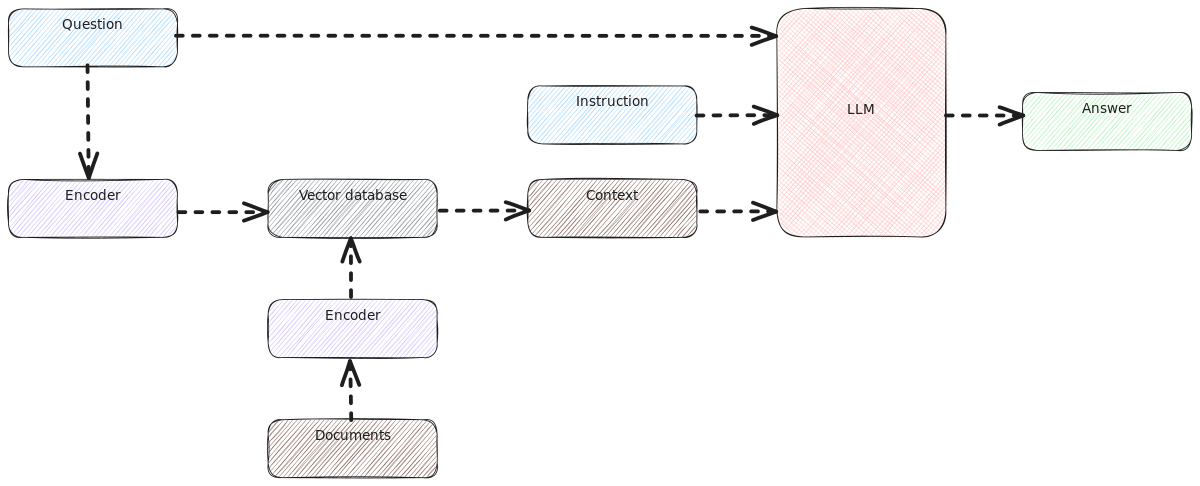
\includegraphics[width=0.9\textwidth]{images/rag.png}
    \caption{Retrieval Augmented Generation pipeline}
    \label{fig:pyanres}
\end{figure}


\chapter{My work}
\section{Crawler}
Before any analysis work can begin, the first sub research question \textit{what are the different archive formats local authorities host in order to comply with the Woo and how are these formats exploited to retrieve as much information as possible?} needs to be answered. 

An overwhelming amount of Dutch local municipalities are allied with one of two service providers that provide archiving, hosting and indexing of past meetings. These two service providers are \href{https://www.ibabs.com}{iBabs} and \href{https://www.notubiz.nl/}{NotuBiz}. Notubiz alone serves over 250 local municipalities, provinces and water authorities, while iBabs serves another TODO. 

Thus, in order to create a service that is compatible with most Dutch (local) government instances, a tool must be developed that is capable of extracting the meetings from at least these two hosting services.

\subsubsection{NotuBiz}
NotuBiz serves many local municipalities in an easy to scrape format. Municipalities have the option to host meetings of different categories and NotuBiz allows for a search to be performed on many different objects such as meeting points, documents, years and meeting types. 

NotuBiz fetches these search results from their server using a GET request. By sniffing the network upon making a search request, I managed to find the endpoint used for search and its necessary parameters. The important keywords are \textit{keywords}, meaning the meeting type, and the \textit{organisations} filter. This organisations filter is especially cumbersome, since it is a municipality specific code used to specify the municipality to be searched. The only way to retrieve this is to make a search request on the desired NotuBiz website and to sniff the network using a dev tool inspector. 

I have created a Python Jupyter Notebook that can scrape any NotuBiz archive with minimal user input needed. Simply the municipality name, the download location, the NotuBiz url, the desired meeting type, the aforementioned unique municipality code and the desired years that the meetings were held. 
The notebook will then find all meetings using Python's Beautiful Soup, writing the meeting page links to a file. When all meeting links are found, they are parsed by Beautiful Soup. When a download link has been found on the page, the video will be downloaded and saved at the appropriate location.

\subsubsection{iBabs}
Municipalities utilizing iBabs for their hosting categorize their meetings into various distinct classifications, which are subsequently subdivided by year.
Each category is listed at the URL 'https://$<$municipality$>$.bestuurlijkeinformatie.nl/Calendar', as seen in figure \ref{fig:ibabsCats}. When a category is chosen, a similar screen allows the user to further specify the year and video.

\begin{figure}
    \centering
    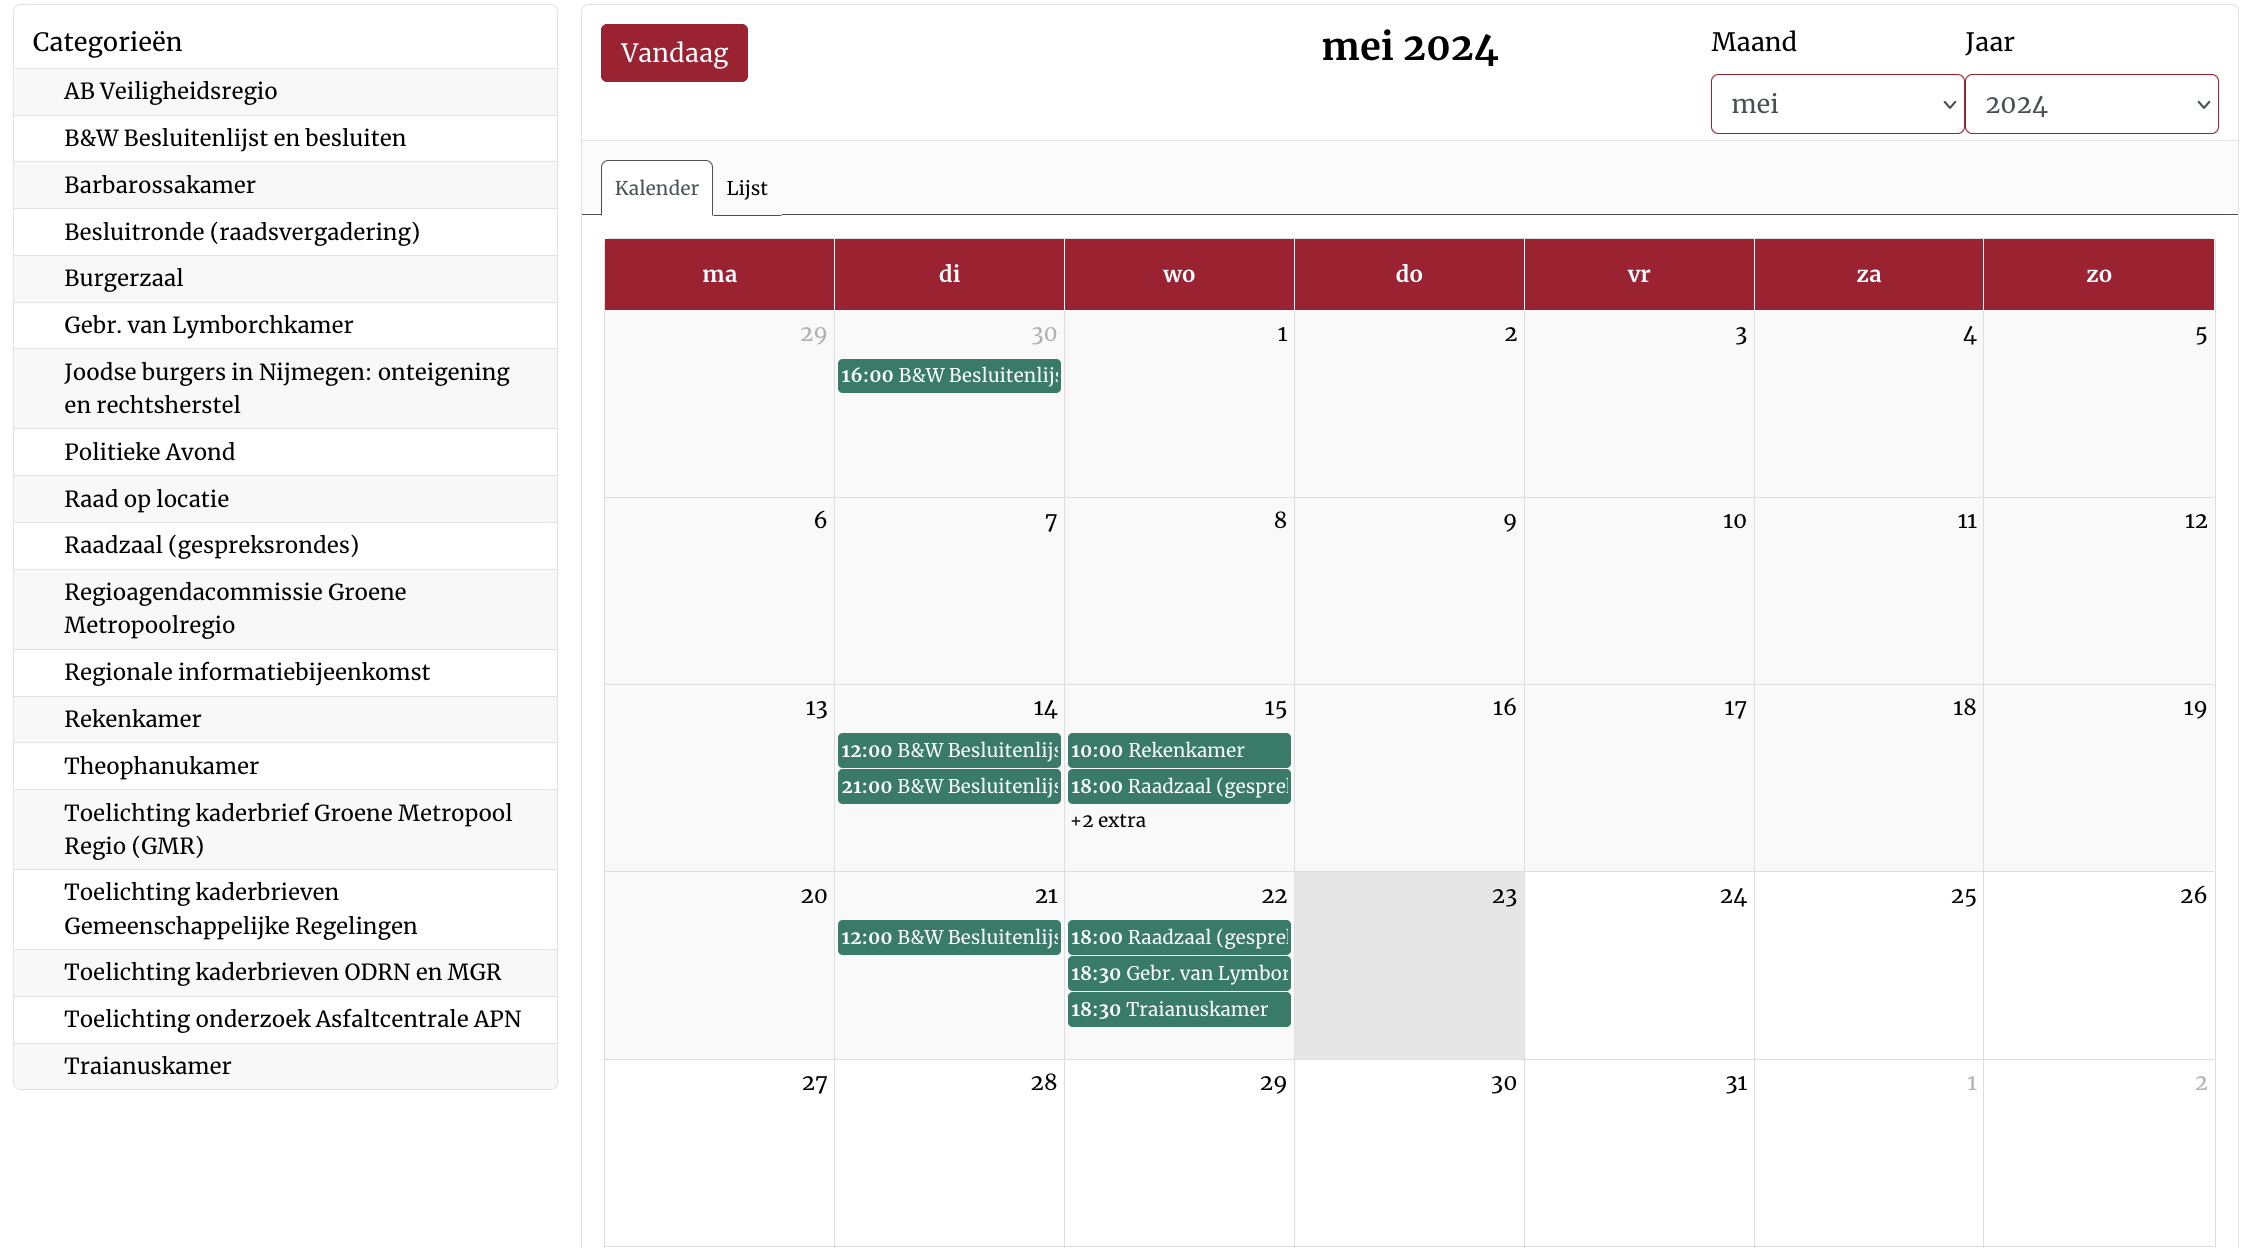
\includegraphics[width=0.95\textwidth]{images/ibabsCats.png}
    \caption{Nijmegen iBabs categories}
    \label{fig:ibabsCats}
\end{figure}

Unlike NotuBiz, iBabs is a dynamically loaded website, meaning data gets loaded in and out of the browser in real-time as users interact with the site. One positive result of this approach is that it enables more responsive and interactive user experiences, as the web page (DOM) can update content without requiring a full page reload. A negative effect is that it makes it more difficult to scrape the webpage for its information and videos.
In addition to this fact, iBabs also uses a specific file format for their video archives, M3U. M3U is not a video file. It is a text file that specifies the locations of parts of a video or audio file hosted on a remote server, allowing for more efficient streaming. This M3U file is only fetched from the server when the user clicks the \textit{play video} button. 

Both these complications mean that static scraping tools and HTML parsers such as Python's urllib and Beautiful Soup are not equipped to deal with the necessities that iBabs requires. To solve these issues, Selenium Web Driver is used. Selenium is an automatable web browser that can be programmed to interact with the DOM, and parse the current web pages. Selenium is also used to sniff the browser's network for the M3U URL that is fetched from the iBabs servers when the \textit{play video} button is clicked. 

I have also written a generic iBabs scraper in the form of a Python Jupyter Notebook. The user only has to specify the municipality name, as seen in the host URL \\ 'https://$<$municipality$>$.bestuurlijkeinformatie.nl/Calendar' and which years should be retrieved. The tool will then fetch all categories that are listen on the home page using Beautiful Soup, creating directories for the municipality, its categories and for each category the different years in the process. 
Next it will use Beautiful Soup to get links to all pages hosting different videos and writes these links URLs to a file dataPath/municipality/category/year/vergaderingen.txt. 
When all video pages have been scraped, Selenium is used to open each page, find and click the \textit{play video} button. After this the browser network is sniffed for the fetched M3U file link which is written to the file dataPath/municipality/category/year/vergaderingenDownloads.txt.

After all M3U URLs have been retrieved, the vergaderingenDownloads.txt file is read and videos are downloaded using a M3U download tool. 


\section{Video analysis}
\subsection{Whisper}
Machine learning is a constantly changing field that evolves rapidly. Every month, dozens of new models and model architectures are released that are more effective in certain situations. 
With this in mind, one of the fundamental principles I uphold is that the design of AI model clients must be as modular as possible. 
This is achieved through the implementation of Python class inheritance. 

In the case of ASR, a base Transcriber class is defined, specifying what methods must be implemented. Then, for each new ASR model, a child class is created where only model specific methods are written. For transcribing, the only model specific method that should be implemented is the \textit{transcribe} method. \textit{transibe} should take in an input path and an output path, which will be used to load the audio file and save the transcription. 
Other methods such as loading transcriptions are model invariant.

As mentioned before, the current state-of-the-art in automatic speech recognition is OpenAI's Whisper. Two Whisper models have been implemented for the final client: one using MLX, a framework allowing fast machine learning on Apple silicon devices, and one using PyTorch. 

\begin{lstlisting}[language=Python, caption={Modular transcriber class implemented in Apple's MLX Whisper port and PyTorch's Whisper port.}]
class Transcriber:
    def transcribe(self, input_file, output_file):
        print("Transcribe method not implemented!")
        return  WhisperReturnCodes.NOT_IMPLEMENTED

    def load_transcription(self, path):
        # Logic which is not specific to any particular model.
        return transcription

class MLX_Transcriber(Transcriber):
    def __init__(self, model):
        self.model = model

    def transcribe(self, input_file, output_file):
        # MLX whisper transcribe logic.
        return

class Torch_Transcriber(Transcriber):
    def __init__(self):
        self.model = whisper.load_model("medium")

    def transcribe(self, input_file, output_file):
        # PyTorch whisper transcribe logic.
        return
\end{lstlisting}

\subsection{Speaker diarisation}
The speaker diarisation client is designed following the same principles and methodologies as those employed in the Whisper client. A base class \textit{Diarisor} defining the model dependant methods is declared, which is used as a parent class by model specific classes, in the case of this project, the \textit{Pyannote} class.

The speaker diarisation client only has two model dependant methods: \textit{diarise} and \textit{embed}. The \textit{diarise} method takes in an input path and an output path, which are used to load the audio and save the generated speaker diarisation output file.

As mentioned in section \ref{sec:pyannote}, pyannote.audio is the current state-of-the-art in the field of speaker segmentation. Because of this, the model used in the final architecture is pyannote.audio V3.2.0, the latest version. In case a new, better model is released, this model can be easily implemented due to the modular design of the client.
\\\\ % otherwise first line of listing is on this page and the rest on the next page, I did not like that

\begin{lstlisting}[language=Python, caption={Modular speaker diarisation class.}]
class Diarisor:
    def diorize(self, input_file, output_file):
        print("Diarize method not implemented!")
        return PyannoteReturnCodes.NOT_IMPLEMENTED

    def embed(self, input_file, from_time, to_time):
        print("Embed method not implemented!")
        return PyannoteReturnCodes.NOT_IMPLEMENTED
\end{lstlisting}

\subsection{Embedder}
Just like the previously mentioned clients, the text embedding client used to embed speaking turns is made in a modular manner, allowing different embed models to be used with ease. Practically all sentence embedding models present day are released on HuggingFace, allowing them to be used through a standard method \textit{encode} in the SentenceTransformers framework developed by HuggingFace. This means that only the class initialisation method is model dependant, while the embed method can be model invariant.

\begin{lstlisting}[language=Python, caption={Modular embed class.}]
class Embedder:
    def __init__(self):
        print("Init method not implemented!")
        return EmbedReturnCodes.NOT_IMPLEMENTED

    def embed(self, text):
        if not self.model:
            return EmbedReturnCodes.NO_MODEL

        return self.model.encode(text)
\end{lstlisting}

Choosing the right embedding model for this project was not as easy as looking at the current leaderboard and selecting the best performing model. The reason for this is the large number of embedding models that are each optimised for different niche use cases. 
The main requirements for this project was that the model needs to be lightweight, quick, and multilingual. Since thousands of hours of video material needs to be embedded, a quick and light model is important. Even more important however, is multilinguality. Multilinguality ensures that semantically similar sentences in different languages will still map close to each other in the vector space. Since most monolingual embedding model are trained on English text, running these models on Dutch sentences will lead to suboptimal performance.

% TODO: Vertellen over hoe ik tot mpnetv2 ben gekomen en de tests ervoor

\subsection{Meeting points}

\section{Retrieval}
\subsection{Weaviate}\label{sec:weaviate}
Unlike the previously mentioned clients, the Weaviate client is not as modular. One of the reasons for this is that releases of new and better database systems are less common that new models. 

The created Weaviate client has methods for various default operations such as creating and deleting collections (similar to tables in relational databases), inserting and deleting entries and getting collection metadata. Besides these basic operations, three search methods from section \ref{retrievalSection} have been implemented: Vector search, BM25 search and Hybrid search.

All search methods allow the user to specify filter parameters such as government, year, speaker and more. Invariant of employed the search method, the client returns data in a uniform format—an array of relevant result objects. Each result object within this array includes properties such as meeting ID, government, year, etc., the result's UUID, its vector representation, and its relevance score.

\subsection{RAG}
RAG consists of two parts: retrieval and generation. A user query is first fed in to the retrieval system which returns one or more pieces of context that are most relevant to the specified query. Next, this context is added to the user query after which a LLM will answer the query using the acquired context. 

The final web app uses a BM25 based retrieval pipeline as specified in section \ref{sec:weaviate}. If no results are found, this is signaled to the user and the process is aborted. In the likely scenario that results are found, the results are added to the query and the LLM is called to answer the question.

Identical to the other clients, the LLM client designed to be modular and easily swapped. The base model only has a single model dependant method: \textit{run}. \textit{run} takes the chat history as an arguments and prompts the LLM. 
In the final product one of two LLM clients are used: A locally running Llama client or a GPT client that calls the OpenAI api. The former can be used on machines that have sufficient RAM and a strong GPU. The latter is recommended for other machines. Since it calls the OpenAI GPT api it is both quick and accurate, bringing with it only a small cost of \$15 per one million output tokens.

\begin{lstlisting}[language=Python, caption={Modular LLM class.}]
class LLM:
    def run(self, history):
        print("run method not implemented!")
        return LLMReturnCodes.NOT_IMPLEMENTED
\end{lstlisting}

\section{Web application}
To make all previously mentioned functionalities accessible to a user, I created a user friendly front end interface using Vue 3.

The web app has two main functionalities, the first being a global search. 
This global search allows the user to search through all available video transcripts. In the case where only a single government, meeting type or year should be searched, selectable filters are present that allow the user to only query specific data.

The other functionality allows the user to navigate to a specific video through the archive by choosing the government, meeting type and year. When a video is selected, the video is shown and playable. 
Below the vide,o different speakers and their speaking turns as well as the meeting discussion points and their times are shown. When a speaker or discussion point is clicked, the video is skipped forward to the clicked timestamp. 
Below the video, a search bar similar to the global search allows the user to search for information in the video. In this video search, both speakers and discussion points can be filtered. 

Next to the video, a LLM powered chat window allows the user to interactively ask questions and information about the video.
\begin{figure}
    \centering
    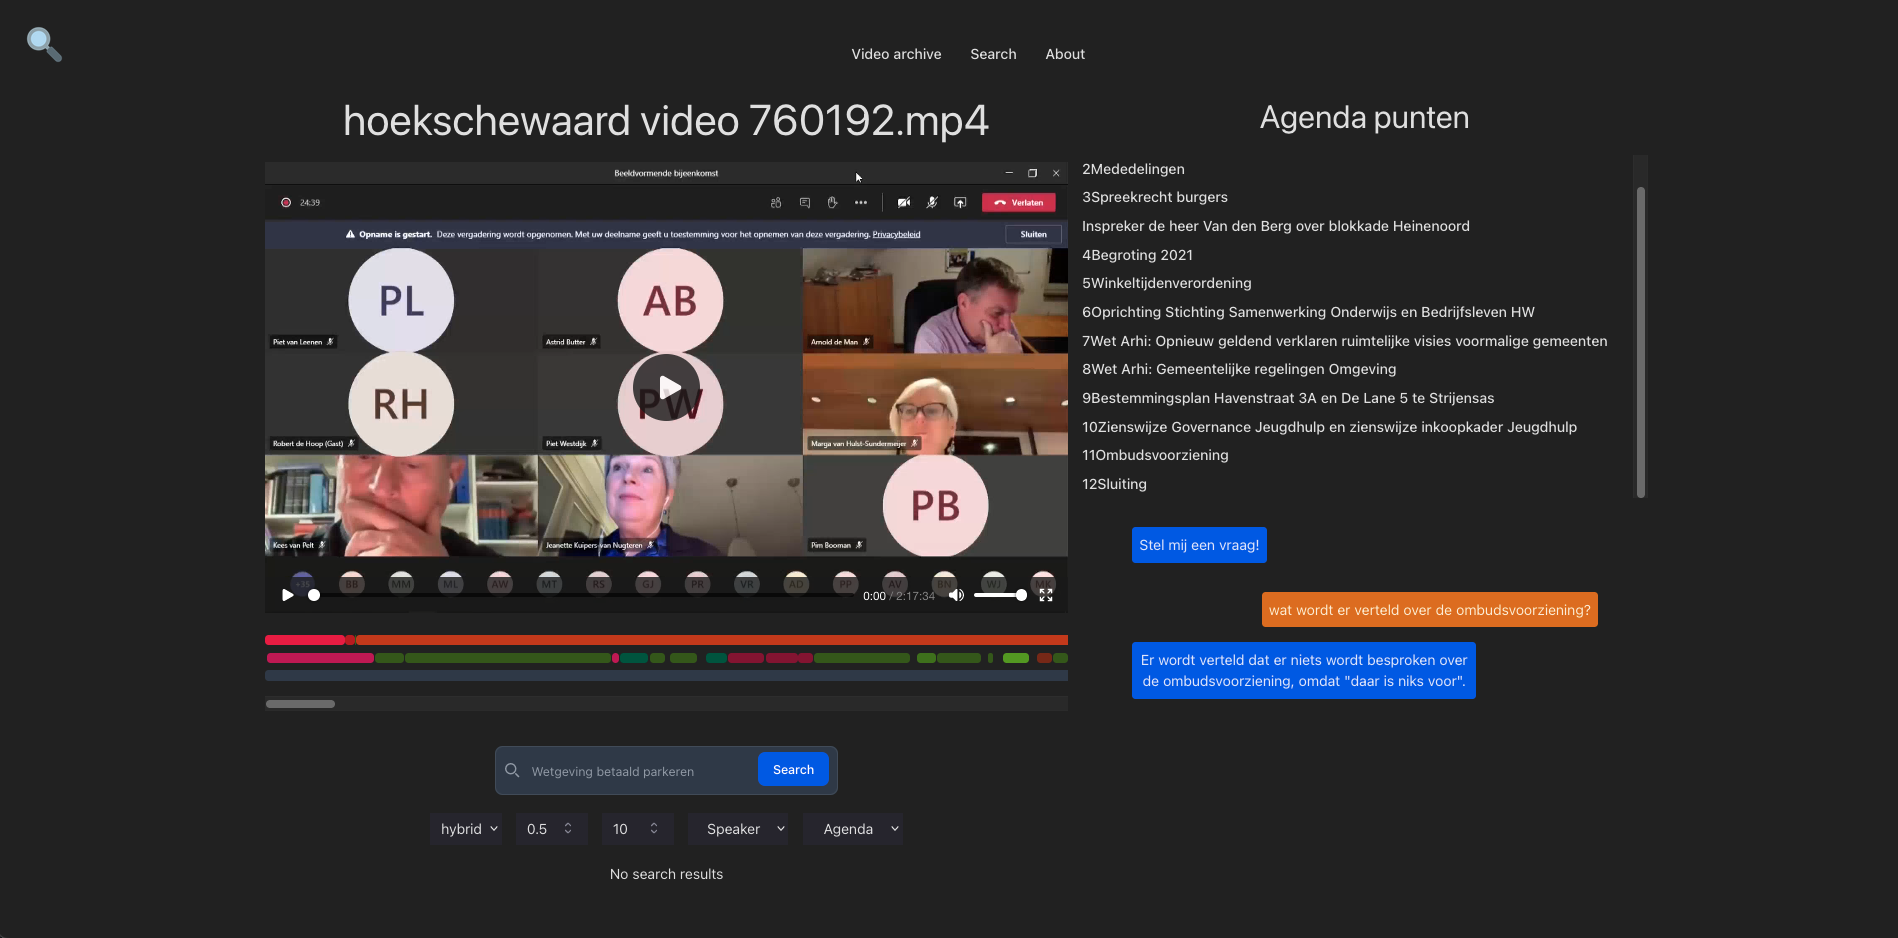
\includegraphics[width=0.9\textwidth]{images/frontend.png}
    \caption{Web application video view}
    \label{fig:frontendVid}
\end{figure}



% \section{Architecture overview}
% Each client described earlier is accessible through a single Python FastAPI server. 
% On startup, this server instantiates the clients, which are then called by the server when requests to certain endpoints are made.

\subsection{Analysis pipeline}
Before a municipality can be added to the archive, all meetings have to be downloaded and analysed. A diagram of the analysis pipeline is shown in figure \ref{fig:pipeline}.

\begin{figure}
    \centering
    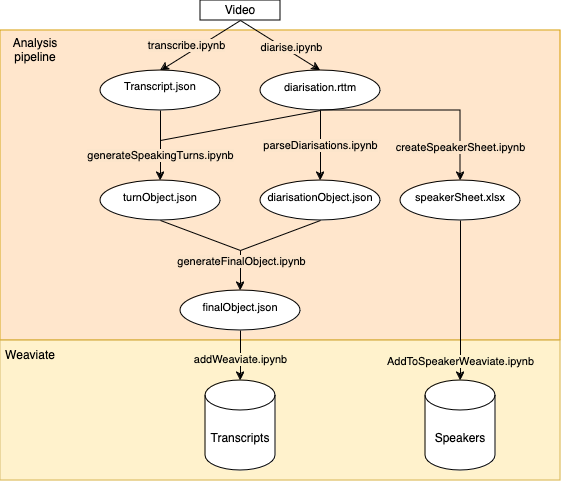
\includegraphics[width=0.85\textwidth]{images/pipeline.png}
    \caption{Video analysis pipeline}
    \label{fig:pipeline}
\end{figure}

The two most important analysis scripts are \textit{transcribe} and \textit{diarise}. These script run Whisper and pyannote respectively, and create a file containing the transcript and diarisation. data. the diarisation data is then used to create a diarisationObject, a JSON file containing the voice profile embedding of each speaker and when they are speaking. Also, a speakerSheet is created. This is and Excel file that an administrator should fill in manually. It maps a detected speaker to a given name, allowing speaker recognition including names. Keep in mind that this should only be done once. Annotated speakers will also be available for videos that were not annotated.

The transcript and diarisation information together are used to create a turnObject. This is a JSON file that contains text of each speaking turn for each speaker and the textual embedding. When this file is created it is combined with the diarisationObject in order to create the final objects that will be added to Weaviate.


\chapter{Experiments}
\section{Crawler}
% Schrijven over hoeveel procent van de meetings correct gedownload worden
\subsubsection{NotuBiz}

\subsubsection{iBabs}
% Schrijven over time out times enzo van selenium om niet te vroeg element not found + subsequent crash te krijen?


\section{Video analysis}
\subsection{Whisper}
The Word Error Rate (WER) (equation \ref{eq:wer}) is a standard metric to evaluate ASR systems. 

To evaluate Whisper's performance on the scraped meetings, I manually transcribed 30 minutes of meetings, selected randomly from five different meetings. To account for structural- and unimportant transcription differences, a normalisation is applied to both the reference and the hypothesis text. 
This normalisation removes all non-alphabetical characters and converts all text to lowercase. 

\begin{figure}
    \centering
    \includegraphics[width=0.85\textwidth]{}
    \caption{Whisper transcription results}
    \label{fig:whisperExperiment}
\end{figure}

\subsection{Pyannote}
As described in section \ref{sec:pyannote}, speaker diarisation is scored based on the Diarisation Error Rate (DER). At the time of writing, pyannote.audio offers the best performing speaker diarisation, as shown in figure \ref{fig:pyanres}. 

To test how well pyannote performs on the municipality dataset, I manually annotated 30 random minutes of meetings, distributed over five different meetings. I used audio tool audacity to obtain millisecond-accurate timestamps. During manual diarisation, speakers were named arbitrarily. After diarisation, the manual speaker names were mapped to the speaker names given by pyannote to make sure the confusion rate metric can be performed.

To address systemic differences in the idea when speech begins and ends, I performed two metrics. One with a 250 milliseconds collar, and one without a collar. 
A collar is a margin of time around each speaker turn boundary. A 250 milliseconds collar would mean that the 125 milliseconds before and after each speaker change are excluded from evaluation.

\begin{figure}
    \centering
    \includegraphics[width=0.85\textwidth]{}
    \caption{pyannote speaker diarisation results}
    \label{fig:pyanExperiment}
\end{figure}

\subsection{RAG}
% Schrijven over rag en hoe goed het is in retrieven in NL
% Hoe lang het duurt voor een response enzo

\subsection{Meeting points}
% Schrijven over dat meeting points niet efficient (en accuraat?) is. Duurt heel lang met LLM enzo

\section{Search engine}
To obtain insights in how well the developed search engine works, I gathered X participants to look for the answer to five questions using five different search methods.

\begin{enumerate}
    \item The contemporary way, scrolling through the video and using its agenda points;
    \item Using the vector search engine;
    \item Using the BM25 search engine;
    \item Using the hybrid search engine;
    \item Using the chat function.
\end{enumerate}

For each participant, the search methods were randomly mapped to a question. 
Each session was recorded so the time taken for each question, any filters used, or other relevant information could be analysed later.

The questions were:
\begin{enumerate}
    \item Wat is de belangrijkste reden die wordt gegeven voor het uitstellen van de harmonisatie van buitensport?
    \item Wat zijn de verwachte voordelen van het installeren van tuintjes rondom ondergrondse containers?
    \item Wat is het verschil tussen het eerste- en het tweede speelterreintje?
    \item Hoe laat wordt de inspreker gewekt door de bromtonen van de nabijliggende windmolens?
    \item Wat is het doel van het voorstel met betrekking tot de gemeenschappelijke regeling van de bedrijfsvoeringspartner?
\end{enumerate}

\chapter{Discussion}
% TODO vertellen dat de cross video speaker recognition aardig werkt (nog kwantificeren hoe goed pr3ecies), alleen bij de corona online meetings werkte het een stuk minder geod, vanwege de irreguliere mics en de hoge gain. Dit betekent dus dat de spreker herkenning gelinkt is aan de (type) mic

% Vertellen dat bij zoom meetings de gain hoger is, waardoor pyannote kleinere fragmenten maakt. Vertellen dat dit niet zozeer een lagere kwaliteit segmentation maakt, maar irregulier vergeleken met een 'normale' meeting die niet op zoom is
% Ook een afbeelding toevoegen van de verschillende gains die het aantoont

% Zeggen dat met whisper de meeste fouten komen door gemompel, wat whisper automatisch eruit filtert (uhh en gemompel dat later duidelijk wordt uitgesproken maar dat heb ik wel uitgeschreven)

\printbibliography

\end{document}
